\section{Results}
\label{sec:results}

\subsection{Final Perplexity After Training}
\label{sec:final_ppl}

\Tabref{tab:main_results} presents per-domain perplexity after 3{,}000 training steps. The curriculum model outperforms the baseline on all 9 core domains, with 5 reaching statistical significance ($p < 0.05$). The baseline wins on all 3 shift domains (expected, since the curriculum model sees them for fewer steps). There is no significant difference on the held-out ArXiv domain.

\begin{table}[t]
\centering
\caption{Per-domain perplexity (mean $\pm$ std over 3 seeds) after 3{,}000 training steps. Lower is better. Best results per domain in \textbf{bold}. $^*$Significant at $p < 0.05$, $^{**}$significant at $p < 0.01$ (paired $t$-test).}
\resizebox{\textwidth}{!}{%
\begin{tabular}{@{}llrrrl@{}}
\toprule
\textbf{Domain} & \textbf{Group} & \textbf{\uniform} & \textbf{\dsc} & \textbf{$\Delta$ PPL} & \textbf{Winner} \\
\midrule
Pile-CC & Core & 270.3 {\scriptsize $\pm$ 2.5} & \textbf{265.0} {\scriptsize $\pm$ 1.3} & $+$5.3 & --- \\
PubMed Abstracts & Core & 214.7 {\scriptsize $\pm$ 2.4} & \textbf{192.1} {\scriptsize $\pm$ 0.8} & $+$22.6$^{**}$ & \dsc \\
StackExchange & Core & 105.7 {\scriptsize $\pm$ 1.2} & \textbf{101.6} {\scriptsize $\pm$ 1.4} & $+$4.1 & --- \\
Github & Core & 60.5 {\scriptsize $\pm$ 0.3} & \textbf{57.9} {\scriptsize $\pm$ 1.7} & $+$2.6 & --- \\
Wikipedia (en) & Core & 358.0 {\scriptsize $\pm$ 2.2} & \textbf{356.6} {\scriptsize $\pm$ 1.0} & $+$1.4 & --- \\
USPTO Backgrounds & Core & 96.1 {\scriptsize $\pm$ 0.4} & \textbf{86.6} {\scriptsize $\pm$ 0.5} & $+$9.5$^{**}$ & \dsc \\
HackerNews & Core & 187.8 {\scriptsize $\pm$ 1.6} & \textbf{178.1} {\scriptsize $\pm$ 0.6} & $+$9.7$^{*}$ & \dsc \\
NIH ExPorter & Core & 150.9 {\scriptsize $\pm$ 1.2} & \textbf{133.5} {\scriptsize $\pm$ 0.6} & $+$17.4$^{**}$ & \dsc \\
Enron Emails & Core & 73.2 {\scriptsize $\pm$ 0.3} & \textbf{66.4} {\scriptsize $\pm$ 0.7} & $+$6.7$^{**}$ & \dsc \\
\midrule
FreeLaw & Shift & \textbf{52.0} {\scriptsize $\pm$ 0.6} & 69.1 {\scriptsize $\pm$ 0.8} & $-$17.1$^{**}$ & \uniform \\
DM Mathematics & Shift & \textbf{8.6} {\scriptsize $\pm$ 0.0} & 11.5 {\scriptsize $\pm$ 0.1} & $-$3.0$^{**}$ & \uniform \\
PubMed Central & Shift & \textbf{84.0} {\scriptsize $\pm$ 1.4} & 98.3 {\scriptsize $\pm$ 0.3} & $-$14.3$^{**}$ & \uniform \\
\midrule
ArXiv & Held-out & \textbf{179.5} {\scriptsize $\pm$ 9.0} & 184.6 {\scriptsize $\pm$ 1.6} & $-$5.1 & --- \\
\bottomrule
\end{tabular}
}
\label{tab:main_results}
\end{table}

\Tabref{tab:group_summary} summarizes these results by domain group. The curriculum model achieves 5.3\% lower average perplexity on core domains but 19.1\% higher perplexity on shift domains.

\begin{table}[t]
\centering
\caption{Average perplexity by domain group. The curriculum model trades shift-domain performance for improved core-domain representations.}
\begin{tabular}{@{}lccc@{}}
\toprule
\textbf{Group} & \textbf{\uniform Avg PPL} & \textbf{\dsc Avg PPL} & \textbf{Advantage} \\
\midrule
Core (9 domains) & 168.6 & \textbf{159.7} & \dsc $+$5.3\% \increase \\
Shift (3 domains) & \textbf{48.2} & 59.7 & \uniform $+$19.1\% \decrease \\
Held-out (1 domain) & 179.5 & 184.6 & --- \\
\bottomrule
\end{tabular}
\label{tab:group_summary}
\end{table}

\subsection{Adaptation Speed}
\label{sec:adapt_results}

\Figref{fig:adaptation} shows the key result. During the 500-step adaptation phase on shift domains, the curriculum model improves 2.8$\times$ faster than the baseline.

\begin{table}[t]
\centering
\caption{Adaptation results over 500 steps of continued training on shift domains. The curriculum model adapts 2.8$\times$ faster and shows less catastrophic forgetting on held-out domains.}
\begin{tabular}{@{}lcc@{}}
\toprule
\textbf{Metric} & \textbf{\uniform} & \textbf{\dsc} \\
\midrule
Initial shift-domain PPL & 47.6 & 57.6 \\
Final shift-domain PPL & 44.4 & 48.5 \\
\textbf{PPL improvement} & 3.3 & \textbf{9.1} \\
\textbf{Improvement ratio} & --- & \textbf{2.8$\times$} \\
Held-out PPL degradation & $-$10.7 & \textbf{$-$7.9} \\
\bottomrule
\end{tabular}
\label{tab:adaptation}
\end{table}

The curriculum model starts with worse shift-domain perplexity (57.6 vs.\ 47.6) but closes the gap much faster: it improves by 9.1 perplexity points compared to just 3.3 for the baseline. Additionally, the curriculum model shows 26\% less degradation on the held-out ArXiv domain during adaptation ($-7.9$ vs.\ $-10.7$ PPL), suggesting some resistance to catastrophic forgetting.

\begin{figure}[t]
    \centering
    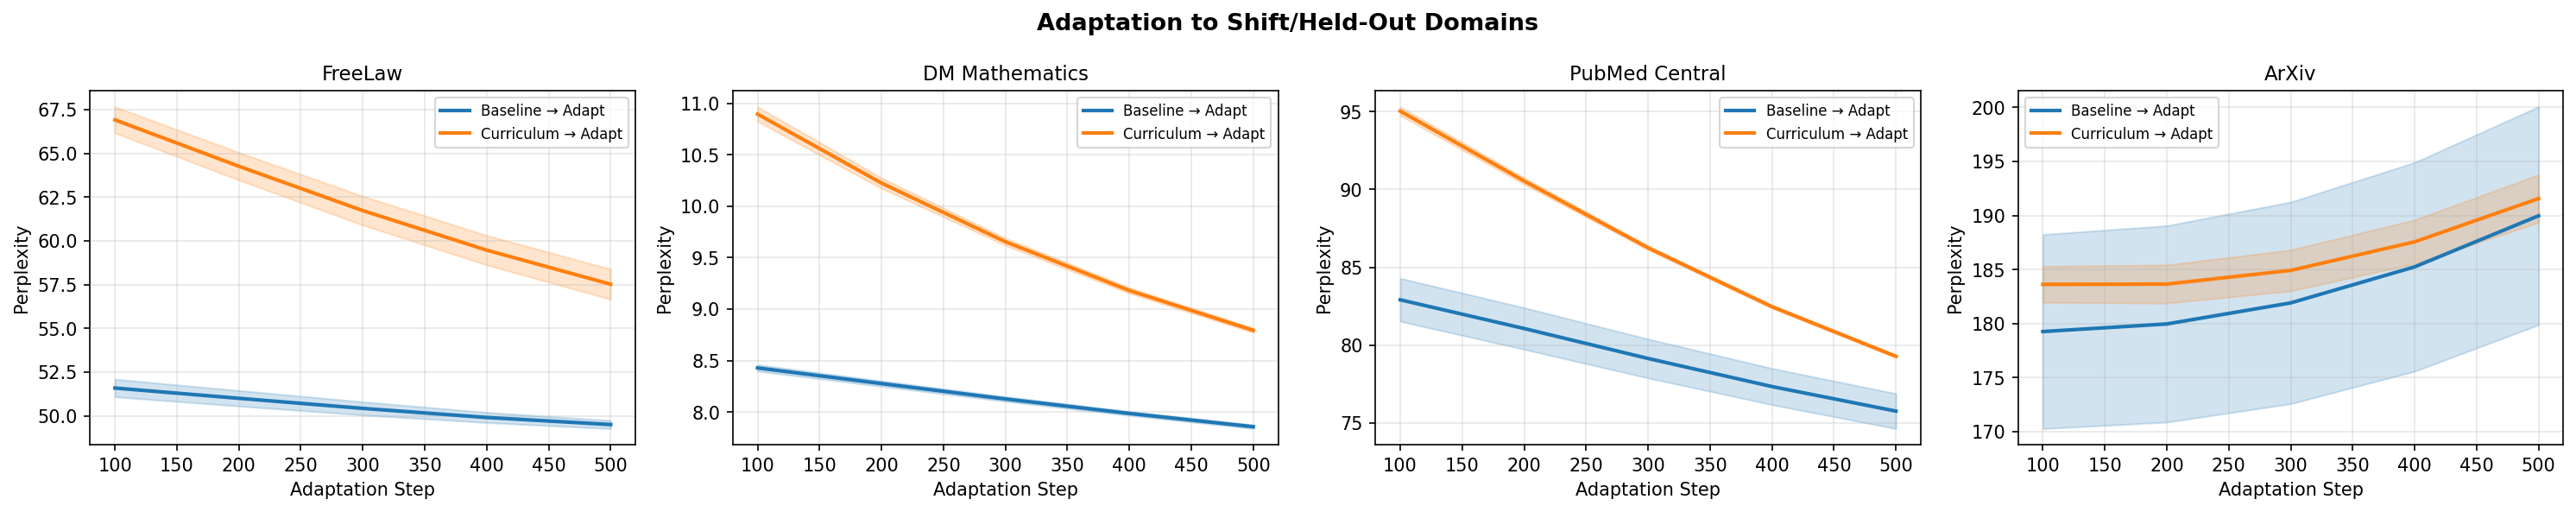
\includegraphics[width=0.95\linewidth]{figures/adaptation_curves.png}
    \caption{Adaptation curves during 500 steps of continued training on shift domains. The \dsc model (orange) improves 2.8$\times$ faster than the \uniform baseline (blue), closing the perplexity gap despite starting from a higher initial value.}
    \label{fig:adaptation}
\end{figure}

\subsection{Training Dynamics}
\label{sec:dynamics}

The training curves reveal several informative patterns (\figref{fig:training_shift} and \figref{fig:final_comparison}).

\para{Transfer without direct training.} During Phase~1, the curriculum model never sees shift-domain data, yet its perplexity on shift domains decreases substantially (from ${\sim}$14{,}000 to ${\sim}$350). This demonstrates significant cross-domain transfer from core domains, though transfer is slower than the baseline's direct training.

\para{Rapid catch-up in Phase~2.} When shift domains are introduced at step 1{,}800, the curriculum model's shift-domain perplexity drops sharply (\eg PubMed Central: 416 $\to$ 98 in 1{,}200 steps). The model does not fully catch up to the baseline, but the convergence rate is notably faster.

\para{Core domain improvement.} The curriculum model consistently outperforms the baseline on core domains by the end of training. We attribute this to Phase~1 concentrating all gradient updates on core domains, yielding stronger representations before the distribution shift occurs.

\begin{figure}[t]
    \centering
    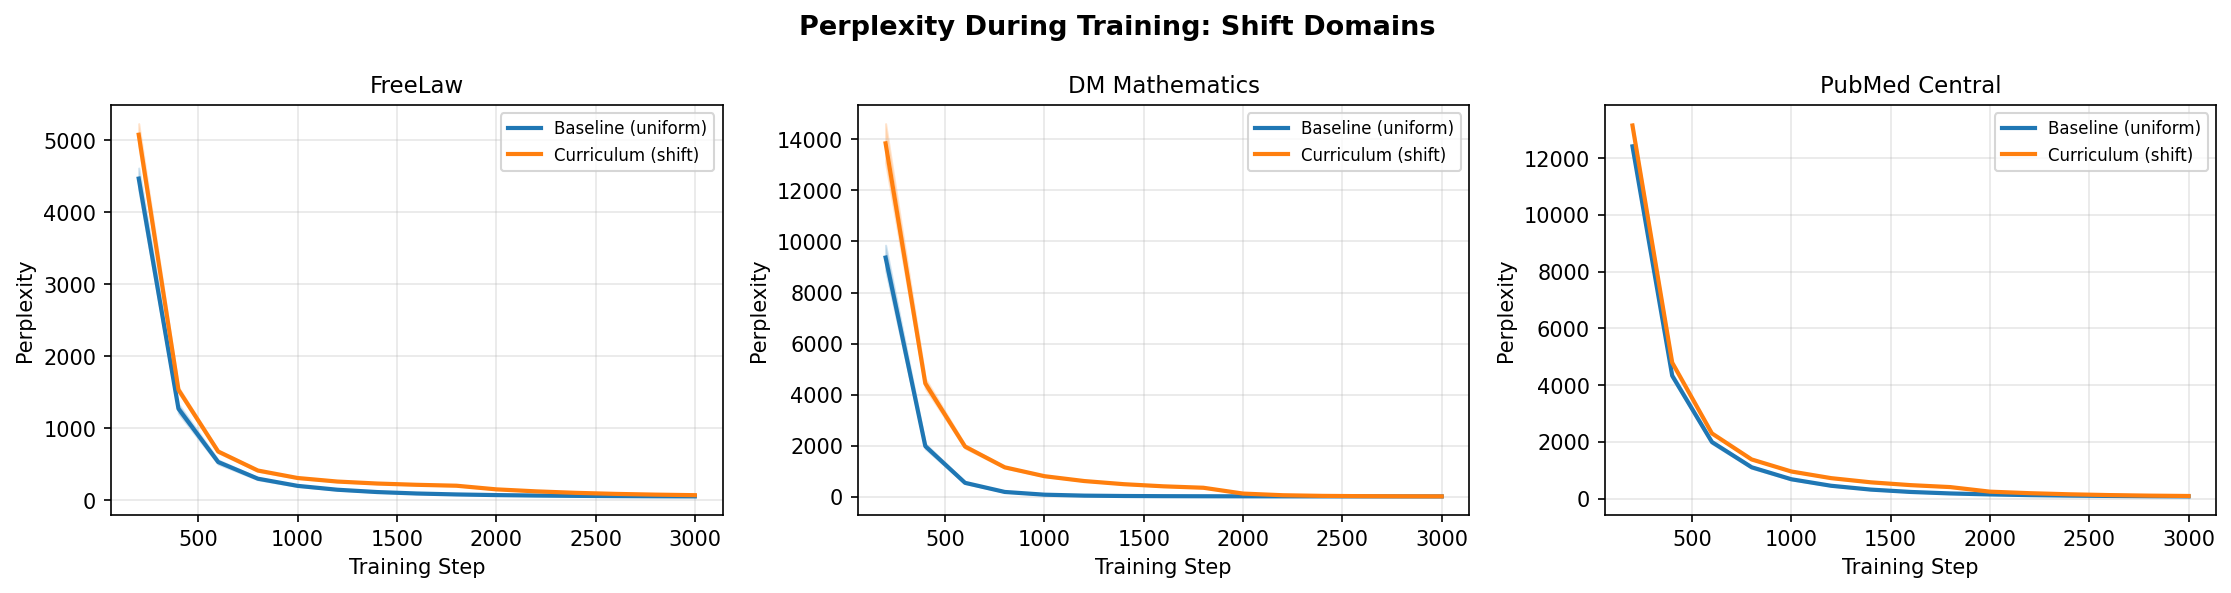
\includegraphics[width=0.95\linewidth]{figures/training_curves_shift_domains.png}
    \caption{Shift-domain training curves. The vertical dashed line marks the Phase~1$\to$Phase~2 transition at step 1{,}800. Before this point, the curriculum model (dashed) improves on shift domains through cross-domain transfer alone. After the transition, it converges rapidly but does not fully catch up to the baseline (solid) within the training budget.}
    \label{fig:training_shift}
\end{figure}

\begin{figure}[t]
    \centering
    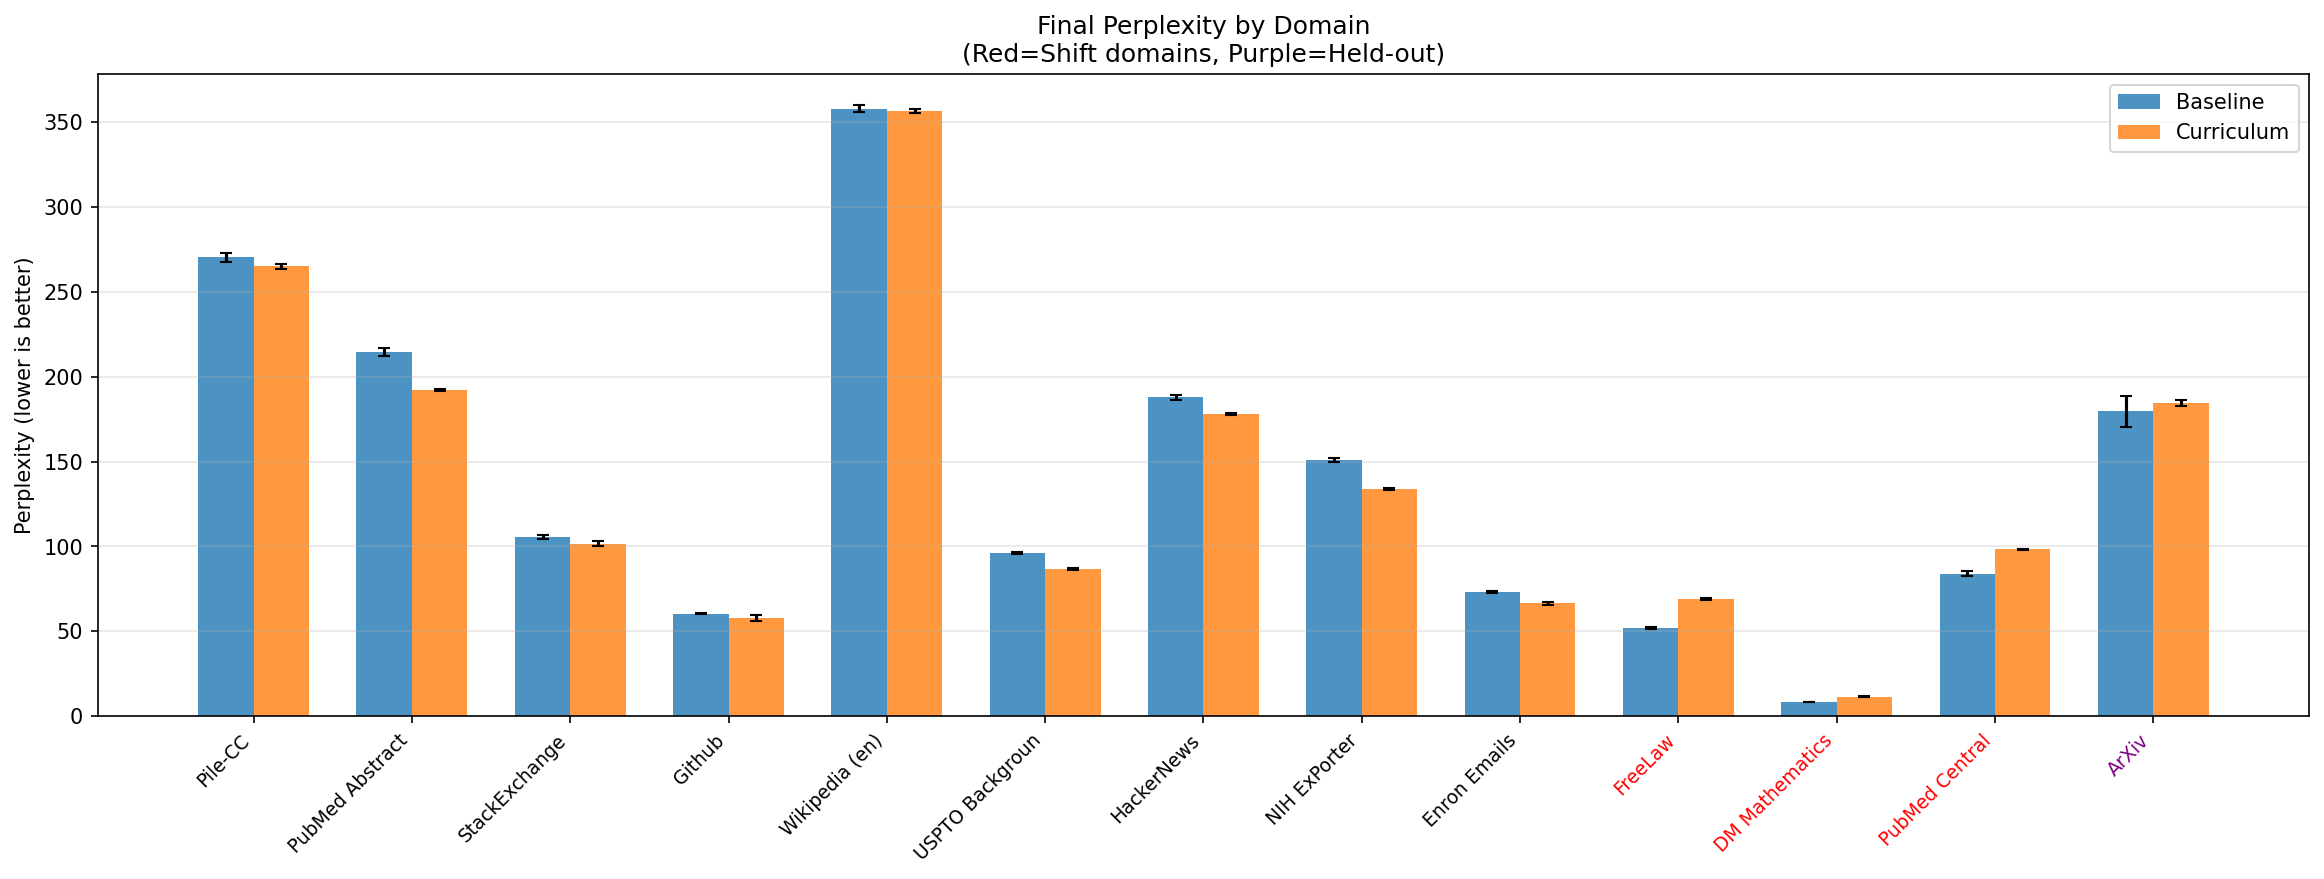
\includegraphics[width=0.95\linewidth]{figures/final_comparison.png}
    \caption{Final perplexity comparison across all 13 domains. The \dsc model (orange) outperforms \uniform (blue) on core domains but underperforms on shift domains. No significant difference on the held-out ArXiv domain.}
    \label{fig:final_comparison}
\end{figure}
